\section{Experimental instructions} \label{subsec:instructions}

\begin{figure}[!htb]
    \centering
    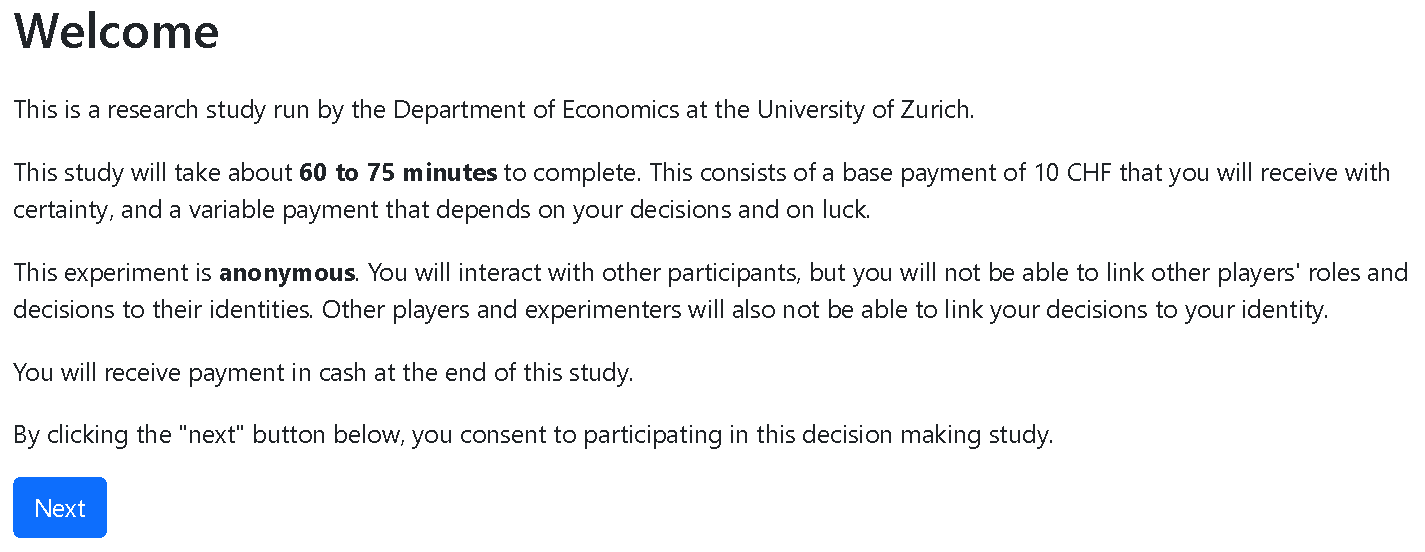
\includegraphics[width=.9\linewidth]{screenshots/welcome.pdf}
    \caption{Welcome screen}
\end{figure}

\begin{figure}[!htb]
    \centering
    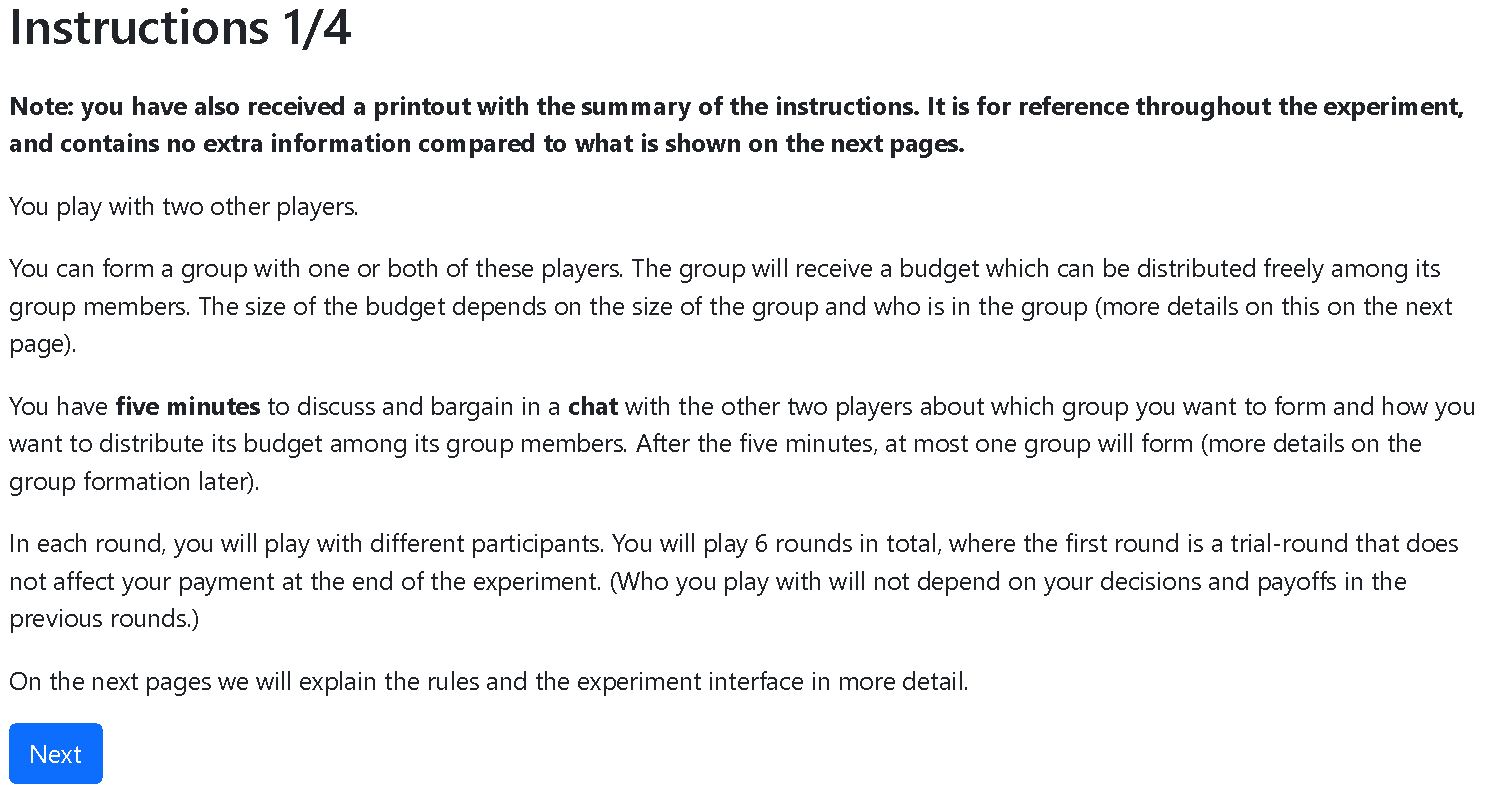
\includegraphics[width=.9\linewidth]{screenshots/instructions_1.pdf}
    \caption{Instructions 1/4: Introduction}
\end{figure}

\begin{figure}[!htb]
    \centering
    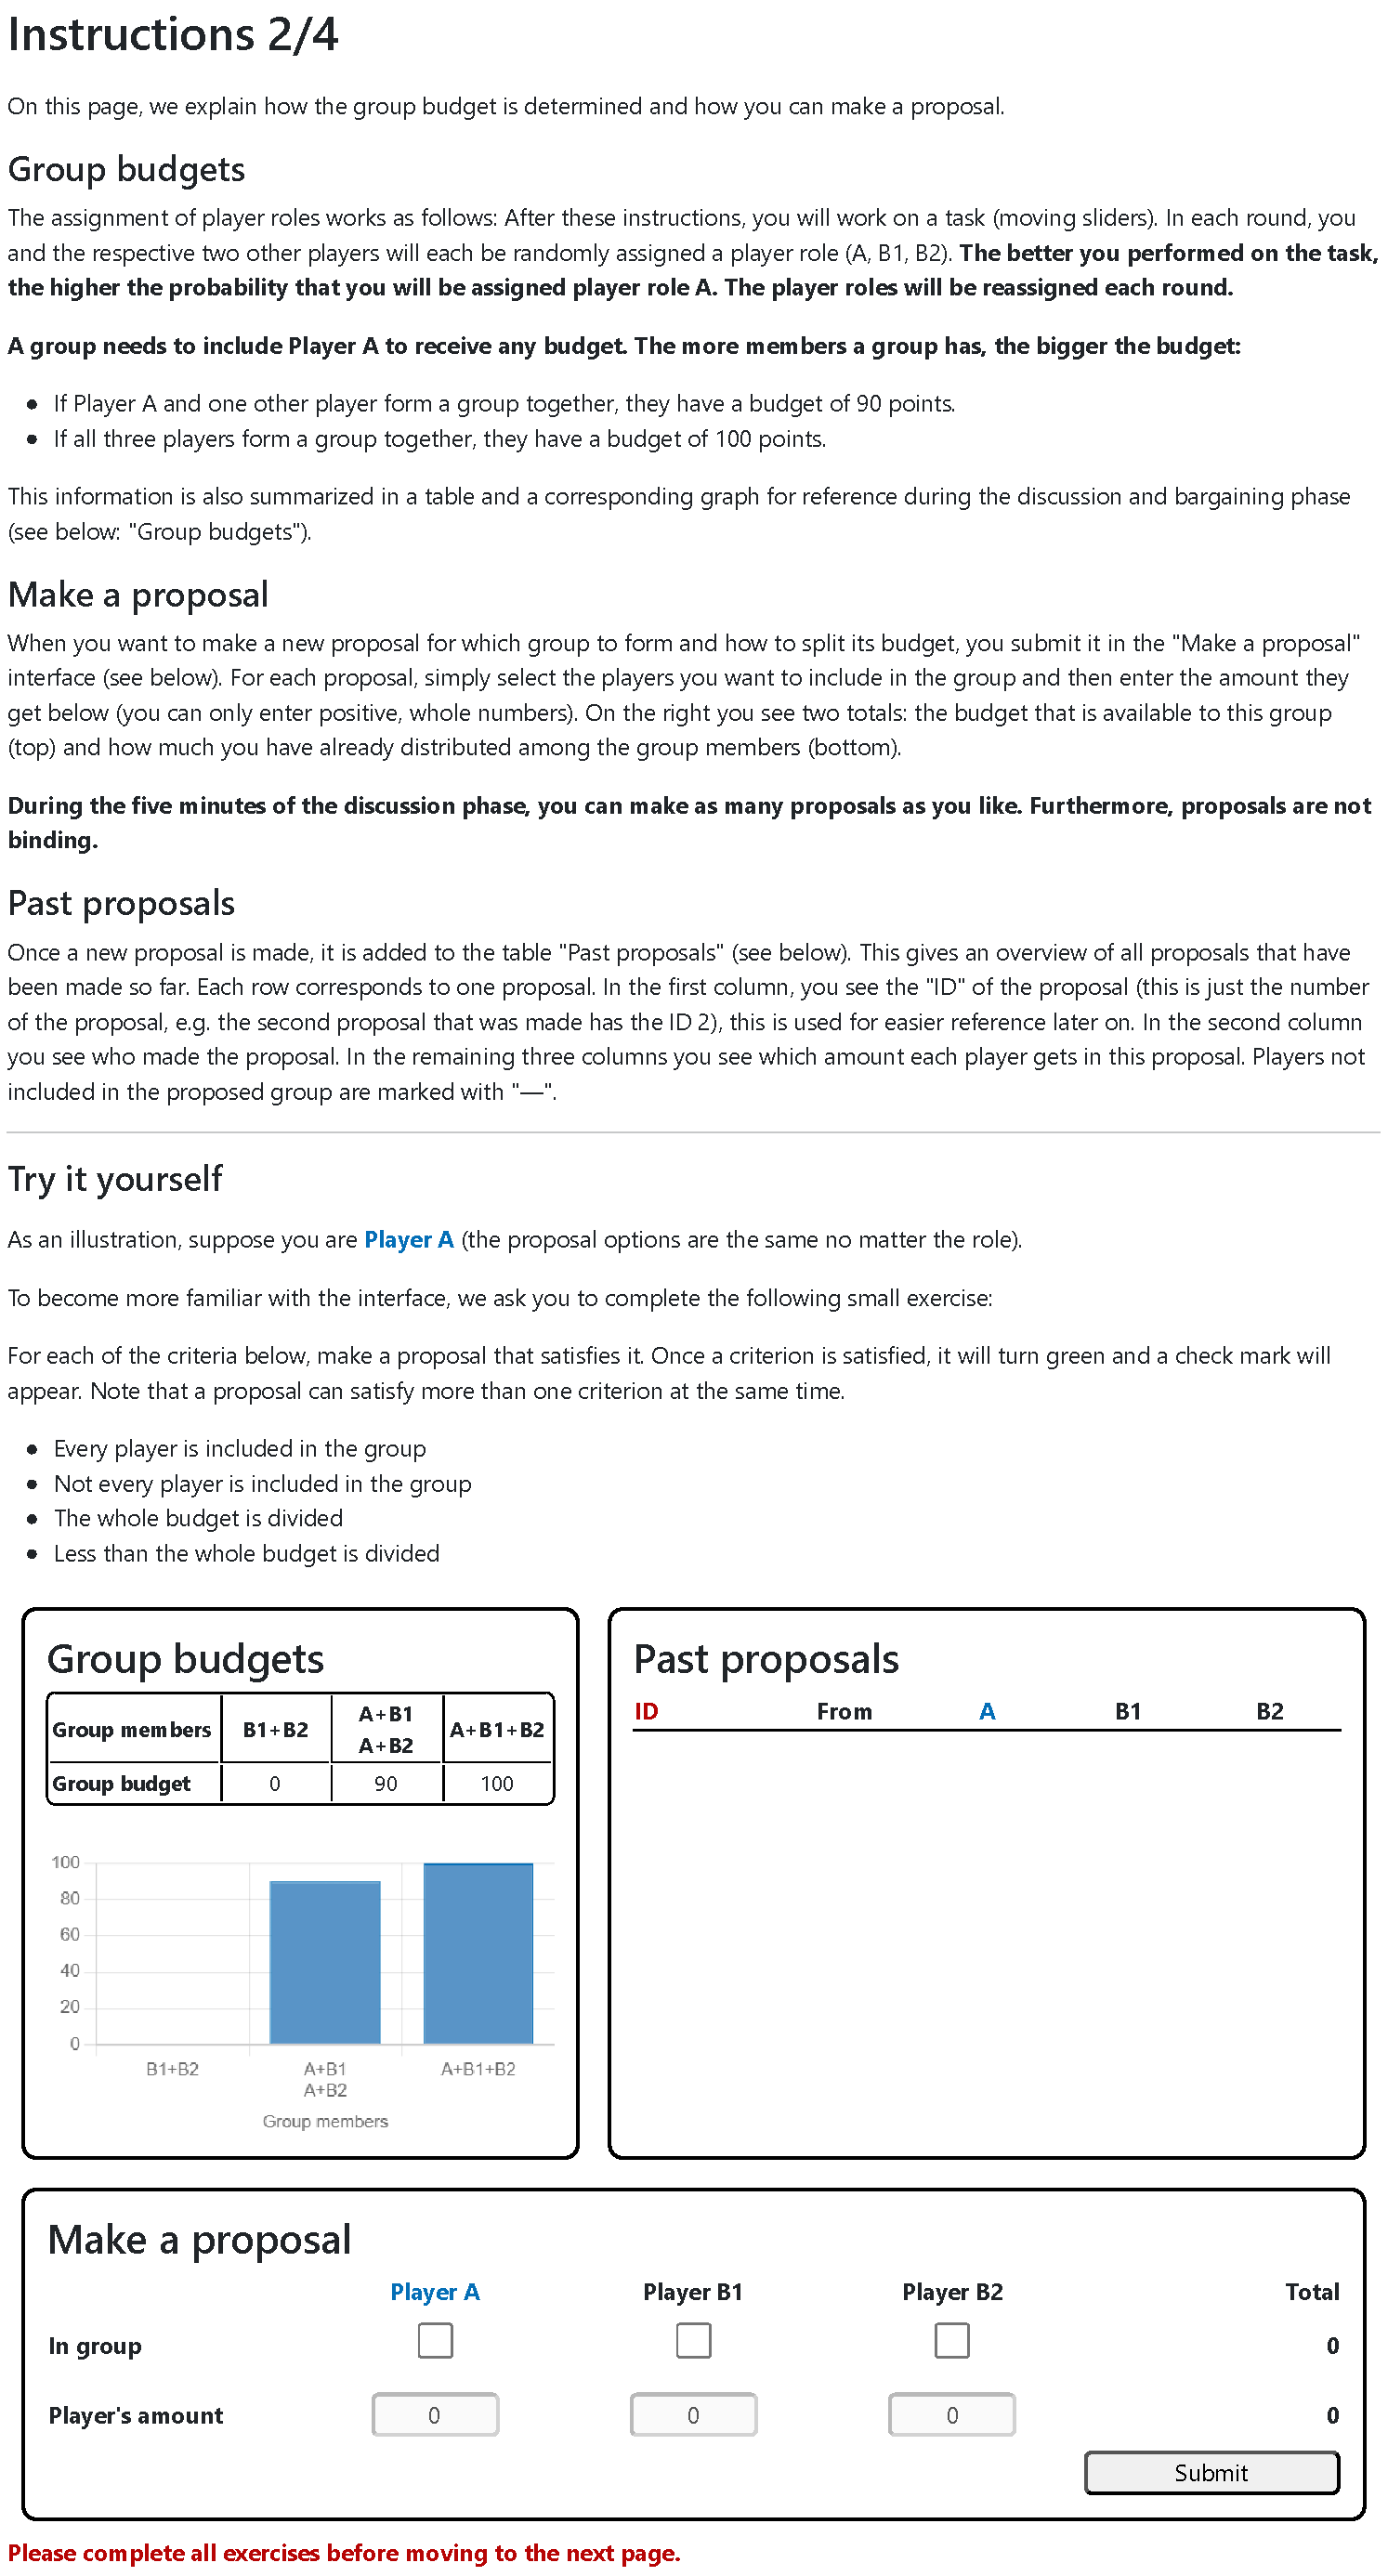
\includegraphics[width=.7\linewidth]{screenshots/instructions_2.pdf}
    \caption{Instructions 2/4: Group budgets}
\end{figure}


\begin{figure}[!htb]
    \centering
    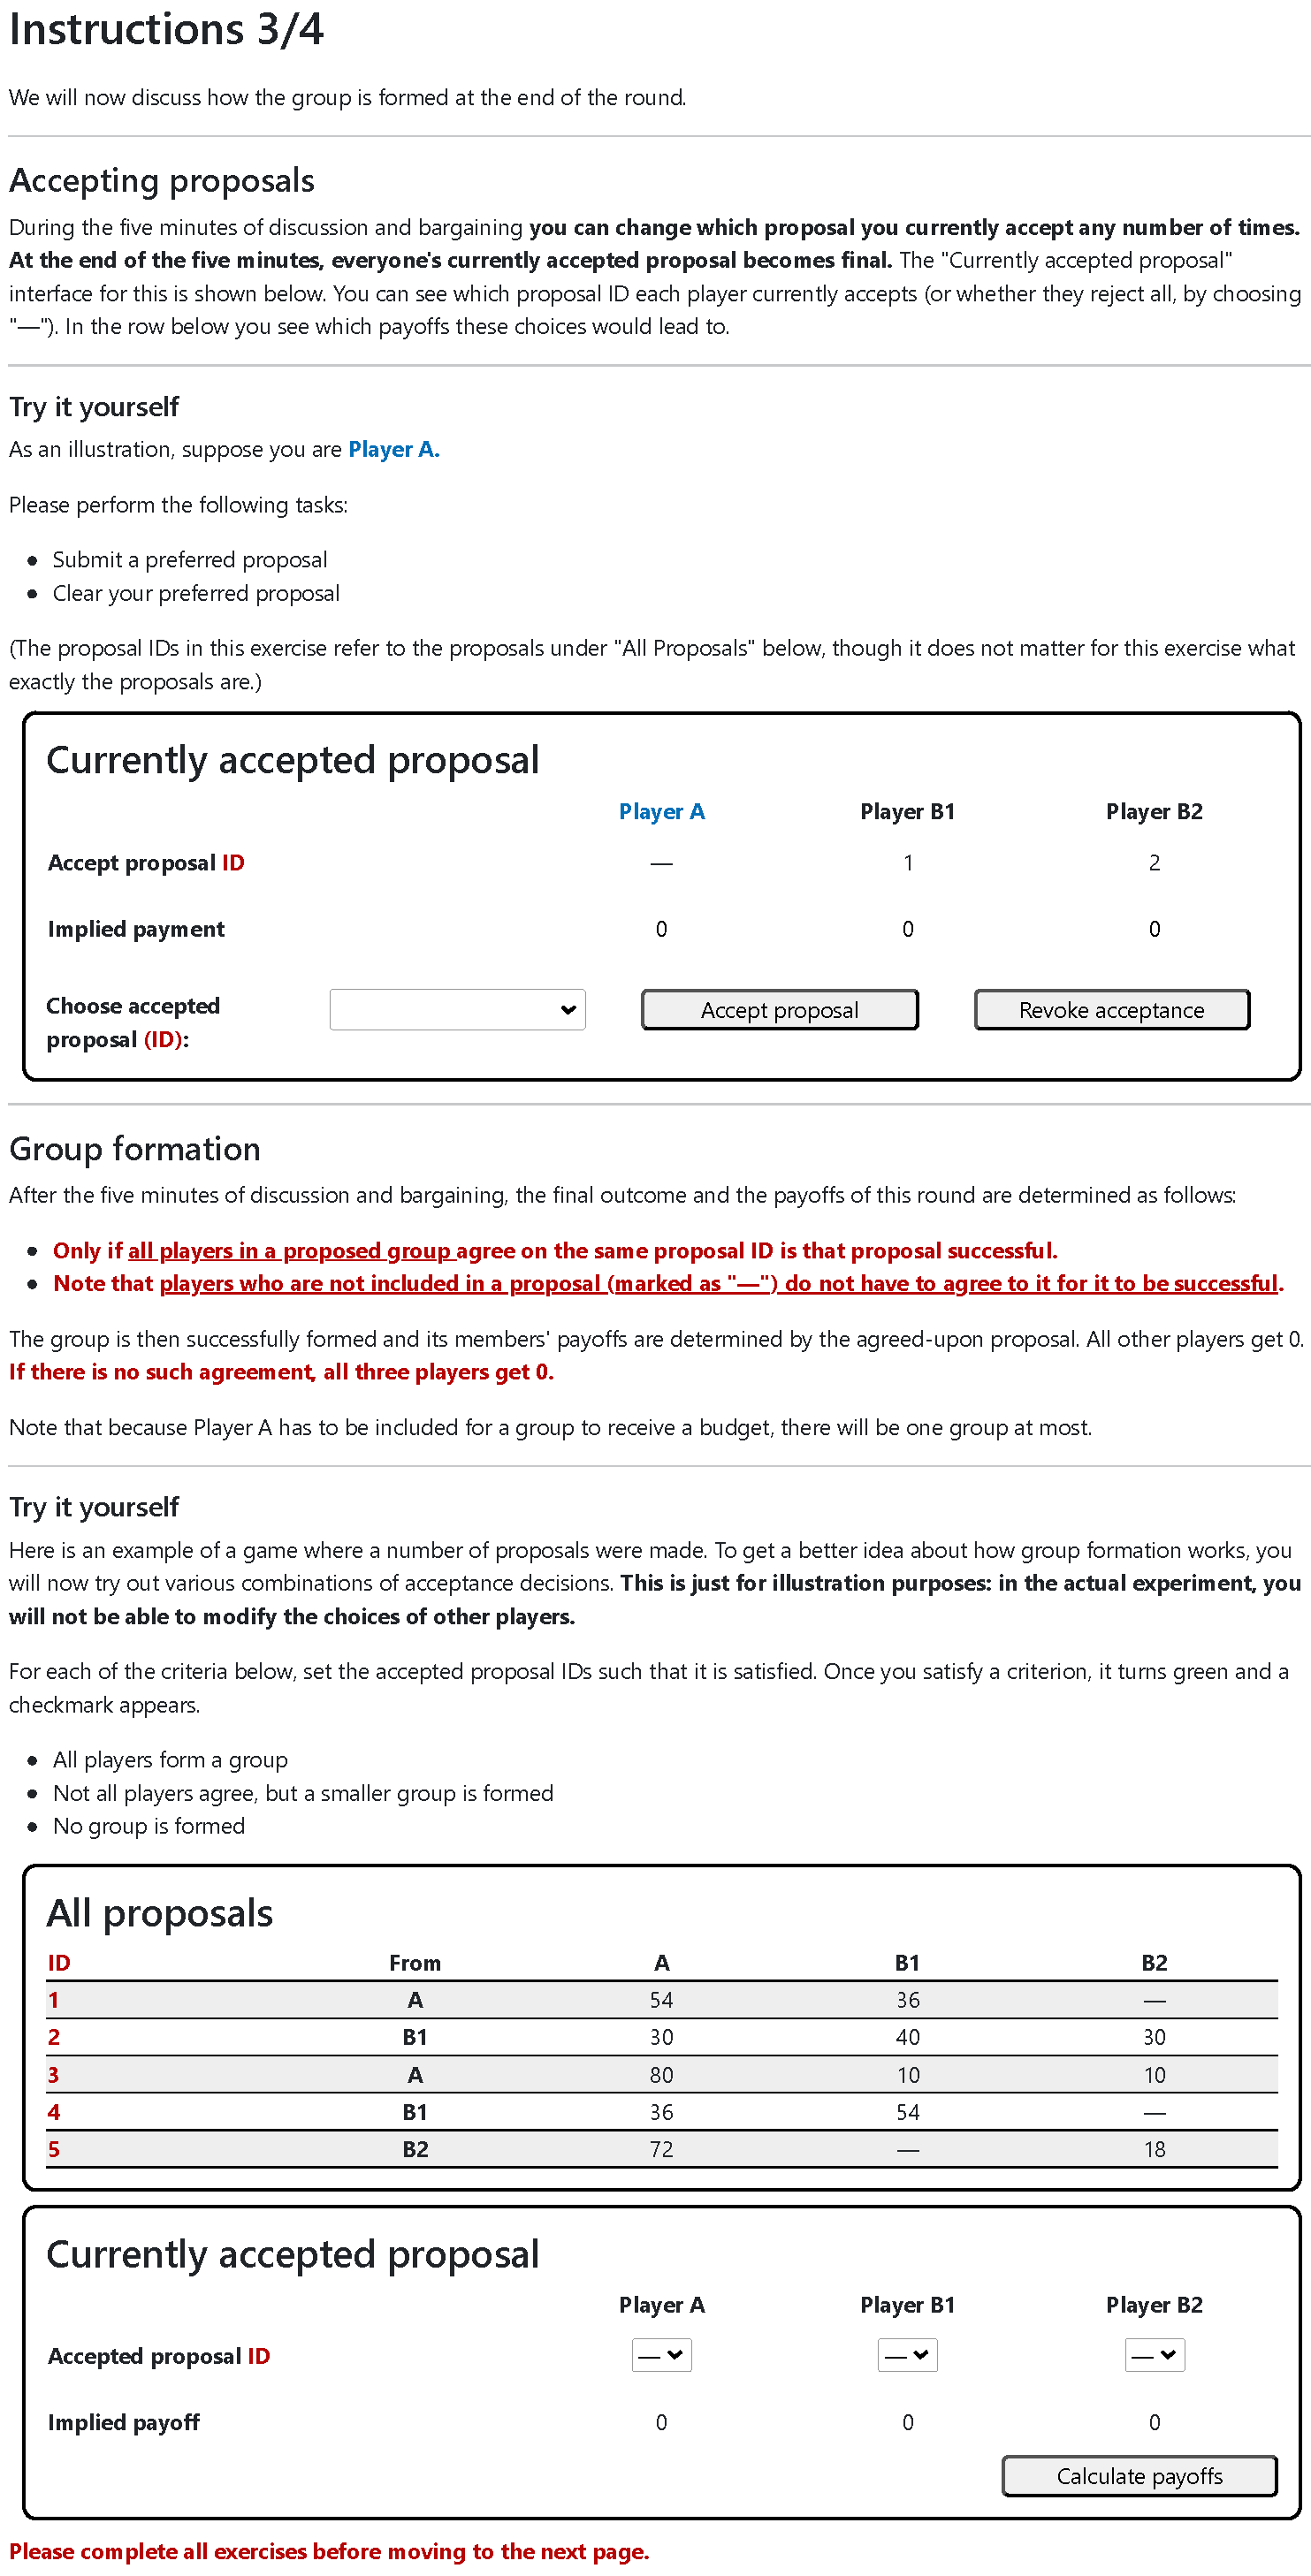
\includegraphics[width=.7\linewidth]{screenshots/instructions_3.pdf}
    \caption{Instructions 3/4: Proposals and group formation}
\end{figure}

\begin{figure}[!htb]
    \centering
    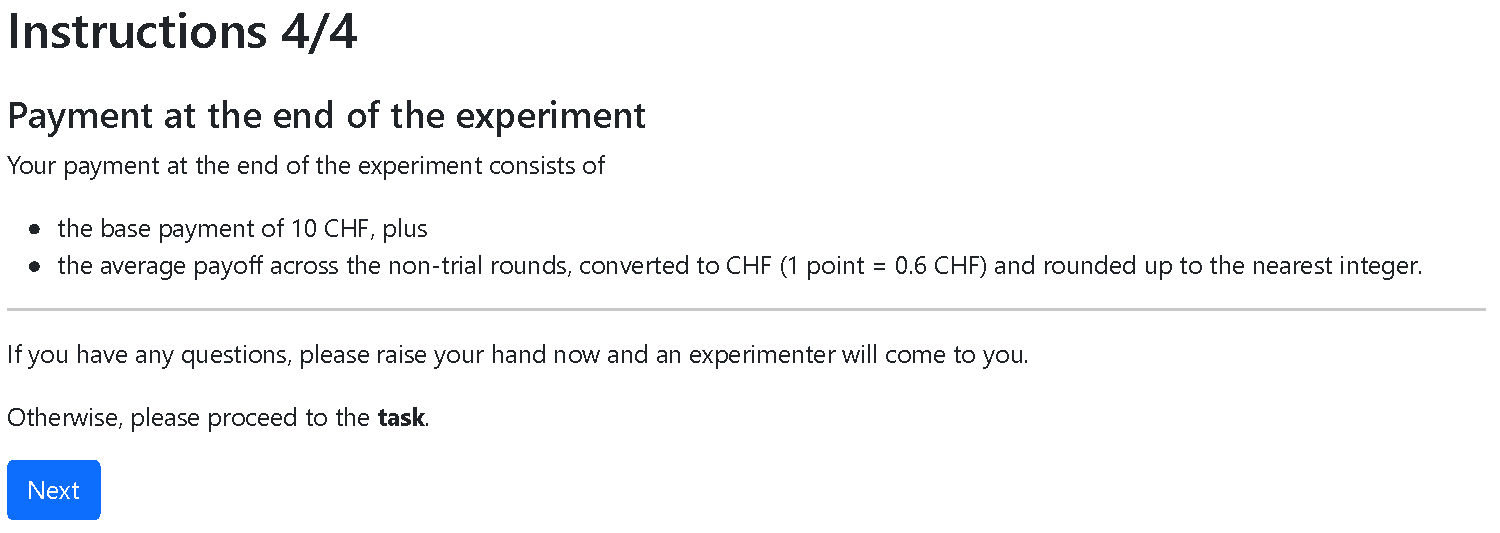
\includegraphics[width=.9\linewidth]{screenshots/instructions_4.pdf}
    \caption{Instructions 4/4: Payment}
\end{figure}


\begin{figure}[!htb]
   \begin{subfigure}[b]{\textwidth}
        \centering
        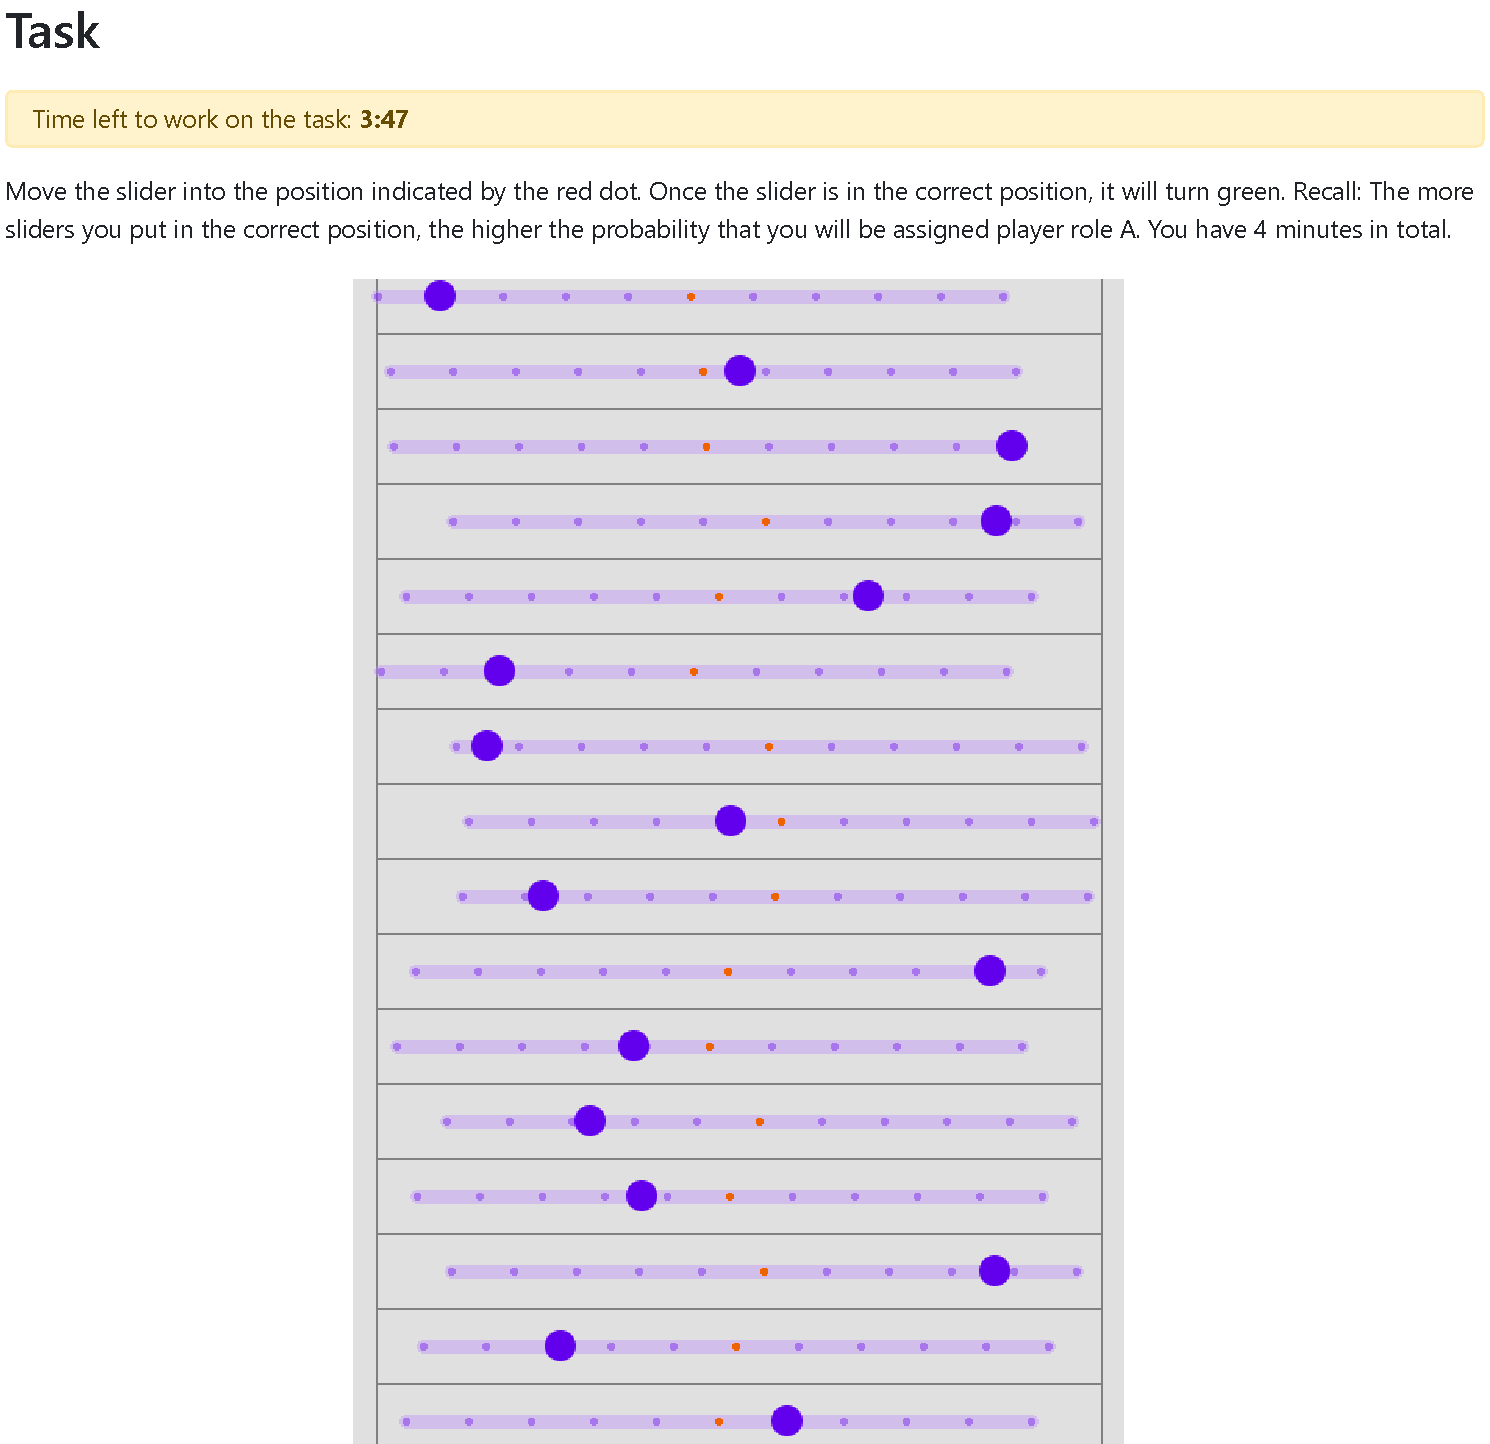
\includegraphics[width=0.9\textwidth]{screenshots/slider.pdf}
    \end{subfigure}
    \par\bigskip
    \begin{subfigure}[b]{\textwidth}
        \centering
        
\includegraphics[width=0.5\textwidth]{screenshots/slider_results.pdf}
    \end{subfigure}
    \caption{Slider task. (Note that this screenshot is cropped, there were 150 sliders in total.)}
\end{figure}

\begin{figure}[!htb]
    \centering
    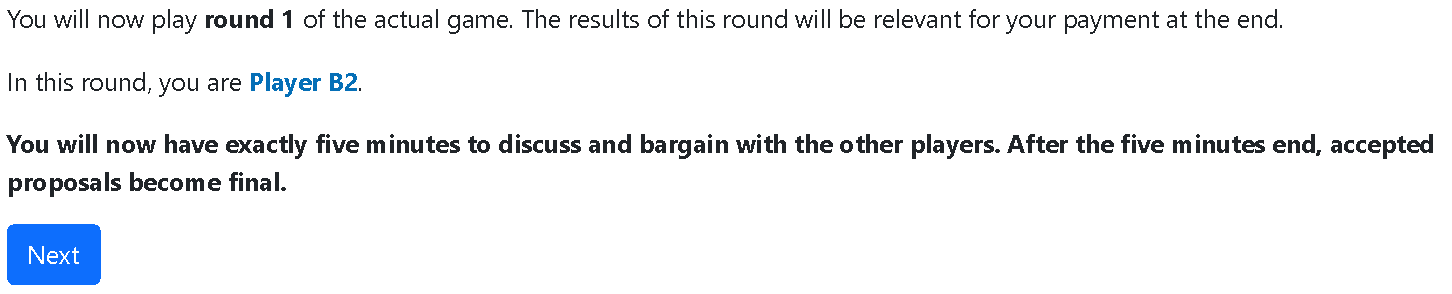
\includegraphics[width=.9\linewidth]{screenshots/info.pdf}
    \caption{Info page before the bargaining round}
\end{figure}

\begin{figure}[!htb]
    \centering
    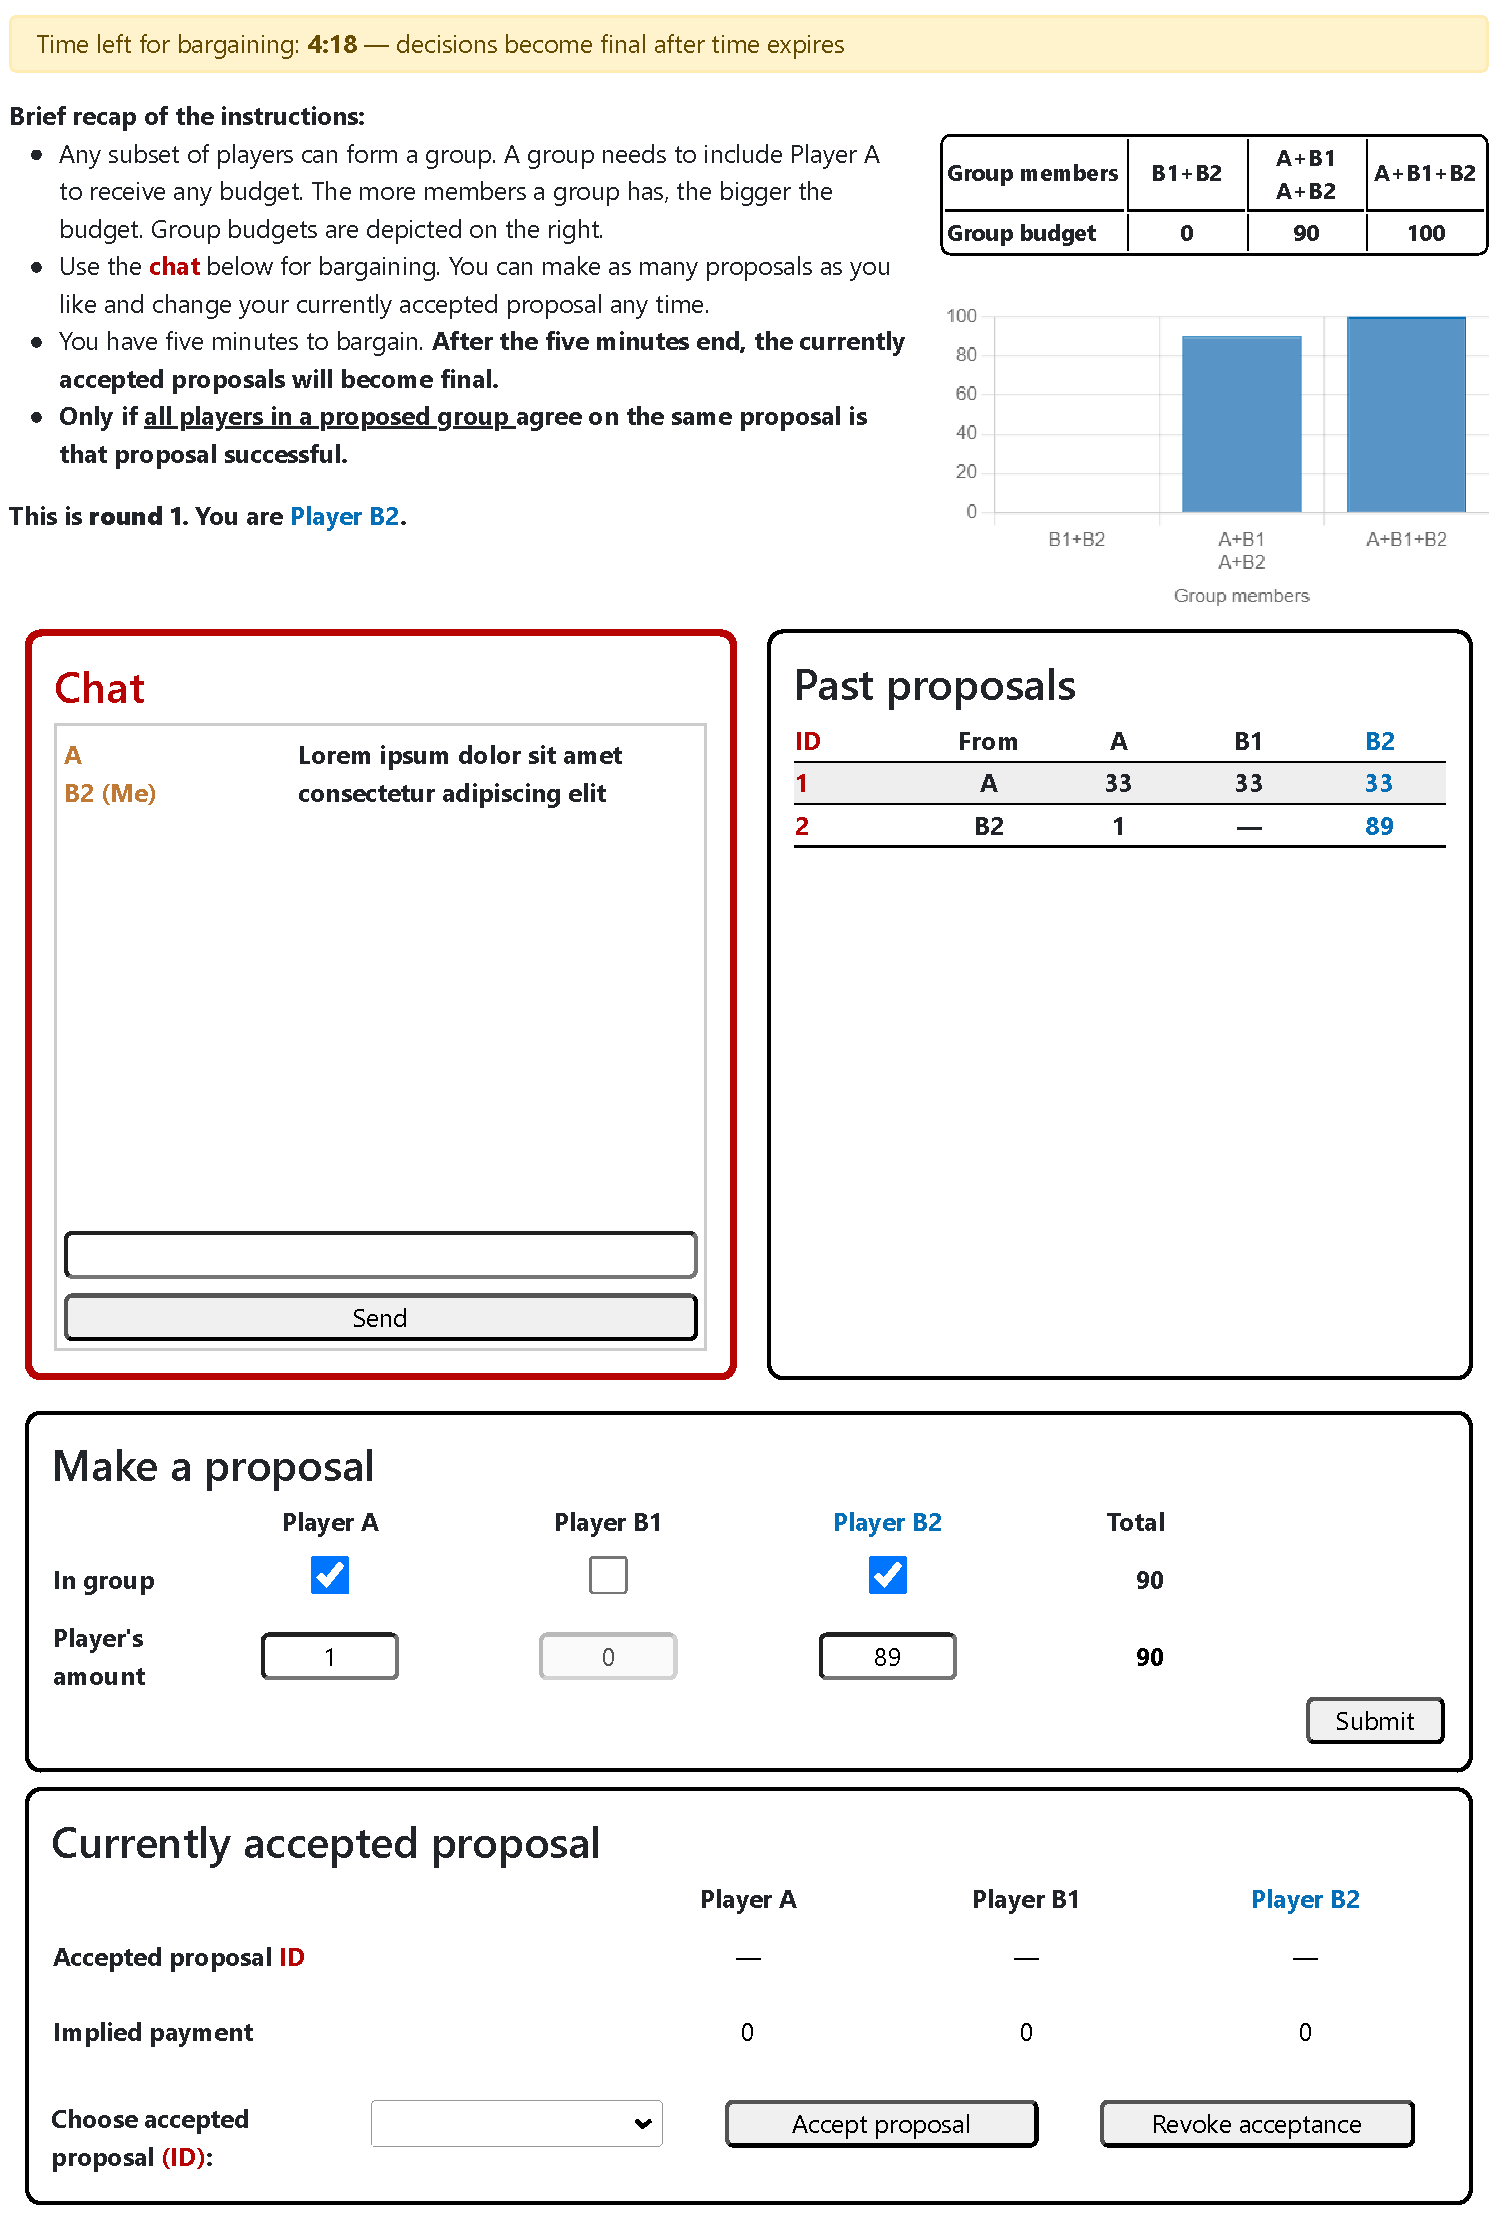
\includegraphics[width=.8\linewidth]{screenshots/bargaining_interface.pdf}
    \caption{Bargaining interface}
    \label{bargaining_interface}
\end{figure}


\section{Chat analysis}

\subsection{Methodology}
\label{sec:gpt_prompt}

To ensure reproducibility as much as possible, the temperature of the GPT-4o model was set to zero. The system prompt we supplied was the following:
\begin{lstlisting}[captionpos=b,caption=System prompt for GPT-4o]
You are going to receive a log containing messages between three players from an economics lab experiment. Players bargained how to split an amount of money. They could additionally use an interface for submitting and accepting proposals. Before the bargaining, players did a slider task and their performance determined their bargaining position.

The log format is the following:
MSG #[MESSAGE_ID] @[PLAYER_NAME]: [MESSAGE]
PROP #[PROPOSAL_ID] @[PLAYER_NAME]: [distribution of the money]
ACC #[ACCEPTANCE_ID] @[PLAYER_NAME]: PROP #[PROPOSAL_ID]
separated by newlines.

Please classify which TOPIC each message (MSG) belongs to. You only have to classify messages, not proposals or acceptances (those latter two are only included for context). The classification should also take into account the context of the message (e.g. when a message is a reply to another).
Each message should be classified into one main and one subtopic. The topics are given in the following nested list:
 - small talk: messages that are not directly related to the experiment
    - greetings and farewells: e.g. saying hello, goodbye, etc.
    - other: e.g. talking about the weather, how to spend the remaining time, etc.
 - bargaining: messages discussing the distribution of the money, making and reacting to proposals, counter-proposals, etc.
    - fairness-based: using arguments based on fairness or justice ideas
    - non-fairness-based: using arguments based on other considerations
 - meta-talk: talking about the experiment itself
    - purpose: discussing what the experimenters are trying to find out
    - rules: discussing and clarifying the rules of the experiment
    - identification: identifying each other, e.g. trying to figure out if players met each other in previous rounds, or identifying information for later

Your response should be of the following format:
#[MESSAGE_ID]: [MAIN_TOPIC], [SUB_TOPIC]
for each message, separated by newlines.
It should look like the contents of a dictionary, but without the surrounding curly braces and apostrophes.
Do not include any other lines, such as code block delimiters or comments.
If there are no rows of type MSG, please respond with NO_MESSAGES without any additional content, such as IDs or comments.
\end{lstlisting}

Then, we supplied the chat, proposal and acceptance history for a given round as the user prompt. An example is given below.
\begin{lstlisting}[captionpos=b,caption=User prompt for GPT-4o]
MSG #1 @A: what are you guys up to?
PROP #1 @B2: A: 34, B1: 33, B2: 33
MSG #2 @A: anyone one split 90 points with me?
MSG #3 @B2: fair play
MSG #4 @B2: propose A
PROP #2 @A: A: 45, B1: 0, B2: 45
ACC #1 @A: PROP #2
MSG #5 @B2: fair i'm down
ACC #2 @B2: PROP #2
MSG #6 @A: i mean if B1 has nothing to say
MSG #7 @A: feel free to offer a better deal :)
MSG #8 @B1: I will not accept it, but i do not think it matters at this point xd
ACC #3 @B1: PROP #0
MSG #9 @A: nope only thing you can do is propose a better deal for me hahah
MSG #10 @A: sorry m8
PROP #3 @B1: A: 46, B1: 44, B2: 0
MSG #11 @A: the power of A
MSG #12 @B1: xdxd no problem
ACC #4 @A: PROP #3
ACC #5 @B1: PROP #3
MSG #13 @A: xD
MSG #14 @A: lets get that game rolling
MSG #15 @A: im sure B2 cannot be happy with that
MSG #16 @B1: hahaha
MSG #17 @B2: :) just wait and see
MSG #18 @A: deal before 10 sek
PROP #4 @B2: A: 50, B1: 0, B2: 40
ACC #6 @B2: PROP #4
ACC #7 @A: PROP #4
\end{lstlisting}

Finally, the model's answer was as follows.
\begin{lstlisting}[captionpos=b,caption=Answer from GPT-4o]
#1: small talk, other
#2: bargaining, non-fairness-based
#3: bargaining, fairness-based
#4: bargaining, non-fairness-based
#5: bargaining, fairness-based
#6: bargaining, non-fairness-based
#7: bargaining, non-fairness-based
#8: bargaining, non-fairness-based
#9: bargaining, non-fairness-based
#10: small talk, other
#11: small talk, other
#12: small talk, other
#13: small talk, other
#14: small talk, other
#15: bargaining, non-fairness-based
#16: small talk, other
#17: small talk, other
#18: bargaining, non-fairness-based
\end{lstlisting}

The results of the categorization of messages is included in the project's git repository along with the raw data.

\subsection{Chat excerpts}
\label{sec:chat_excerpts}

This section contains a number of chat excerpts (including proposals and acceptance decisions) to illustrate some more common themes we observed when reviewing the chat logs. They are presented mostly to give an idea about the kind of textual data we obtained from the experiment.

\begin{figure}[!htb]
    \centering
    \begin{subfigure}[b]{0.42\textwidth}
        \centering
        \includegraphics[width=\linewidth]{out/figures/chat_excerpt-5640,5647-5648,5660-5663.pdf}
        \caption{Treatment $Y=30$: discussing that partial agreement makes no sense}
        \label{fig:chat_stability_y30}
    \end{subfigure}
    \hspace{0.1\textwidth}
    \begin{subfigure}[b]{0.42\textwidth}
        \centering
        \includegraphics[width=\linewidth]{out/figures/chat_excerpt-6846-6847,6849,6851,6853,6855,6857,6859.pdf}
        \caption{Treatment $Y=90$: making the small players compete}
        \label{fig:chat_stability_y90}
    \end{subfigure}
    \caption{Examples of stability-based reasoning from the chat logs. Note, that some messages have been omitted.}
    \label{fig:chat_stability}
\end{figure}

\begin{figure}[!htb]
    \centering
    \begin{subfigure}[b]{0.42\textwidth}
        \centering
        \includegraphics[width=\linewidth]{out/figures/chat_excerpt-7052,7054,7057-7063.pdf}
        \caption{Treatment $Y=90$:, agreeing on almost equal split}
        \label{fig:chat_fairness_equal_split}
    \end{subfigure}
    \hspace{0.1\textwidth}
    \begin{subfigure}[b]{0.42\textwidth}
        \centering
        \includegraphics[width=\linewidth]{out/figures/chat_excerpt-7894-7901,7906.pdf}
        \caption{Treatment $Y=90$: rejecting unequal proposals}
        \label{fig:chat_fairness_reject_small}
    \end{subfigure}
    \caption{Examples of fairness-based reasoning from the chat logs. Note that some messages have been omitted for brevity.}
    \label{fig:chat_fairness}
\end{figure}

\begin{figure}[!htb]
    \centering
    \begin{subfigure}[b]{0.42\textwidth}
        \centering
        \includegraphics[width=\linewidth]{out/figures/chat_excerpt-6508-6509,6511,6513,6524,6527,6528-6529.pdf}
        \caption{Discussing the impact of having the ability to chat with each other}
        \label{fig:chat_meta_chat}
    \end{subfigure}
    \hspace{0.1\textwidth}
    \begin{subfigure}[b]{0.42\textwidth}
        \centering
        \includegraphics[width=\linewidth]{out/figures/chat_excerpt-5501-5508.pdf}
        \caption{Small talk and feedback about the length of the rounds}
        \label{fig:chat_meta_time}
    \end{subfigure}
    \caption{Examples of discussing the experiment from the chat logs. Note that some messages have been omitted for brevity.}
    \label{fig:chat_meta}
\end{figure}

\section{Payoffs by matching group}

\begin{figure}[!htb]
    \centering
    \includegraphics[width=1\linewidth]{out/figures/payoff_matching_group_average_rounds_all.pdf}
    \caption{Average payoff on the matching-group level by role and treatment. (There were six matching groups à six subjects in each treatment.)}
    \label{fig:matching_group}
\end{figure}

\section{Reciprocity concerns}

\begin{figure}[!htb]
    \centering
    \begin{subfigure}[b]{0.49\textwidth}
        \centering
        \includegraphics[width=\textwidth]{out/figures/payoff_average_rounds_[2,3,4,5].pdf}
        \caption{Rounds 1-4}
    \end{subfigure}
    \hfill
    \begin{subfigure}[b]{0.49\textwidth}
        \centering
        \includegraphics[width=\textwidth]{out/figures/payoff_average_rounds_[6].pdf}
        \caption{Round 5}
    \end{subfigure}
    \caption{Average payoffs for each player role by treatment, for the given rounds. Vertical bars denote 95\% confidence intervals for the within-group means.}
    \label{fig:reciprocity}
\end{figure}

A potential concern is that reciprocity is a driver of behavior and leads to more equal payoffs: for example, people might give a non-zero payoff to the dummy player because they expect to be the dummy player in later rounds, or they might agree on outcomes closer to the equal split because they expect to be a small player in later rounds. This is corroborated by the fact that some subjects try to identify each other (\Cref{fig:chat_topics_all}). While a large part of it is due to small talk about topics such as countries of origin or degrees, some subjects tried to agree on code words in order to identify each in later rounds, for example in order to find out if groups were actually reshuffled. Reciprocity, however, would suggest that the behavior in the last round is different from the previous rounds. While we can not exclude that reciprocity is a factor, the comparison of the average payoffs of the last rounds versus all other non-trial rounds does not indicate any substantial difference.

\section{Survey: axioms}

\begin{figure}[!htb]
    \centering
    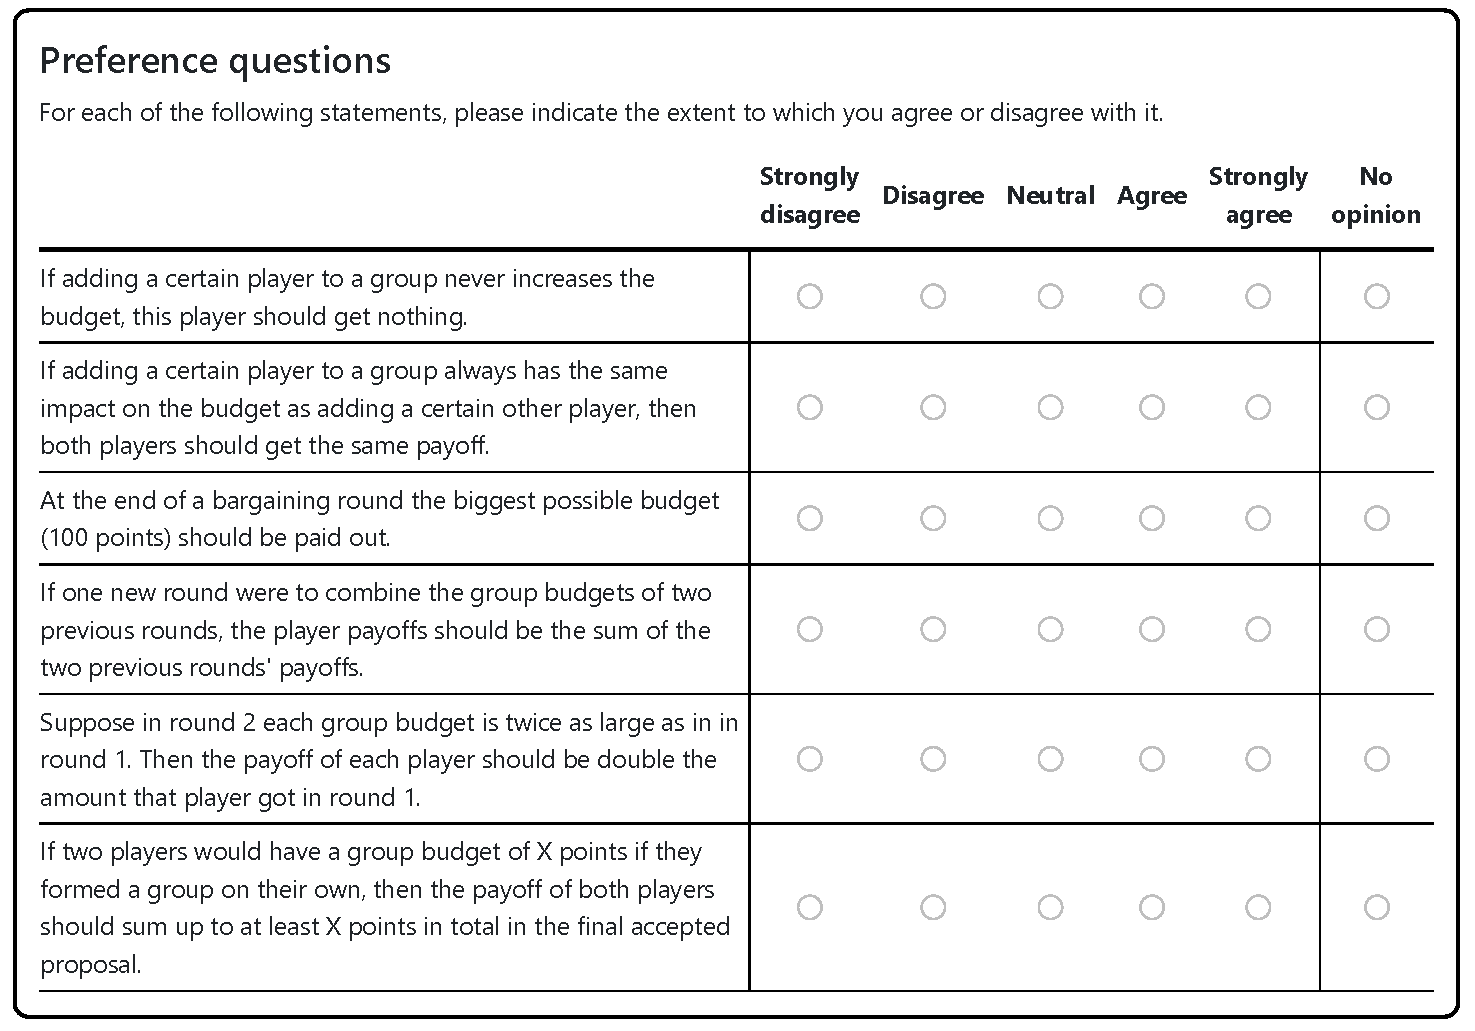
\includegraphics[width=.9\linewidth]{screenshots/survey_axioms.pdf}
    \caption{Survey questions for the axioms}
    \label{fig:survey_axioms_questions}
\end{figure}



\begin{figure}
    \centering
    \includegraphics[width=.99\linewidth]{out/figures/axioms_survey_efficiency.pdf}
    \includegraphics[width=.99\linewidth]{out/figures/axioms_survey_symmetry.pdf}
    \includegraphics[width=.99\linewidth]{out/figures/axioms_survey_linearity_additivity.pdf}
    \includegraphics[width=.99\linewidth]{out/figures/axioms_survey_linearity_HD1.pdf}
    \caption{Survey: empirical support of the axioms}
    \label{fig:axioms_survey_1}
\end{figure}

\begin{figure}
    \ContinuedFloat
    \centering
    \includegraphics[width=.99\linewidth]{out/figures/axioms_survey_dummy_player.pdf}
    \includegraphics[width=.99\linewidth]{out/figures/axioms_survey_stability.pdf}
    \caption{Survey: empirical support of the axioms}
    \label{fig:axioms_survey_2}
\end{figure}


\begin{figure}
    \centering
    \includegraphics[width=1\linewidth]{out/figures/allocations_proposals_by_dummy_player_axiom.pdf}
    \caption{Proposals by agreement with the dummy player axiom.}
    \label{fig:axioms_proposals_dummy_player}
\end{figure}

\begin{figure}
    \centering
    \includegraphics[width=1\linewidth]{out/figures/allocations_proposals_by_symmetry_axiom.pdf}
    \caption{Proposals by agreement with the symmetry axiom.}
    \label{fig:axioms_proposals_symmetry}
\end{figure}

\begin{figure}
    \centering
    \includegraphics[width=1\linewidth]{out/figures/allocations_proposals_by_efficiency_axiom.pdf}
    \caption{Proposals by agreement with the efficiency axiom.}
    \label{fig:axioms_proposals_efficiency}
\end{figure}

\begin{figure}
    \centering
    \includegraphics[width=1\linewidth]{out/figures/allocations_proposals_by_linearity_HD1_axiom.pdf}
    \caption{Proposals by agreement with the linearity (homogeneity of degree 1) axiom.}
    \label{fig:axioms_proposals_linearity_HD1}
\end{figure}

\begin{figure}
    \centering
    \includegraphics[width=1\linewidth]{out/figures/allocations_proposals_by_linearity_additivity_axiom.pdf}
    \caption{Proposals by agreement with the linearity (additivity) axiom.}
    \label{fig:axioms_proposals_linearity_additivity}
\end{figure}

\begin{figure}
    \centering
    \includegraphics[width=1\linewidth]{out/figures/allocations_proposals_by_stability_axiom.pdf}
    \caption{Proposals by agreement with the stability axiom.}
    \label{fig:axioms_proposals_stability}
\end{figure}

\section{Subject sample: Population characteristics} 

\begin{figure}[!h]
    %\centering
    \begin{subfigure}[b]{0.49\textwidth}
        \centering
        \includegraphics[width=\textwidth]{out/figures/survey_gender.pdf}
        \caption{Gender composition, by treatment.}
        \label{fig:balance_gender}
    \end{subfigure}
    \hfill
    \begin{subfigure}[b]{0.49\textwidth}
        \centering
        \includegraphics[width=\textwidth]{out/figures/survey_degree.pdf}
        \caption{Degree composition, by treatment.}
        \label{fig:balance_degree}
    \end{subfigure}
    \vfill
    \begin{subfigure}[b]{0.43\textwidth}
         \centering
        \includegraphics[width=\textwidth]{out/figures/survey_age.pdf}
        \caption{Average age, by treatment.}
        \label{fig:balance_age}
    \end{subfigure}
    \label{fig:balance}
\end{figure}

\begin{figure}
    \ContinuedFloat
    \centering
    \begin{subfigure}[b]{\textwidth}
        \centering
        \includegraphics[width=1\textwidth]{out/figures/survey_nationality.pdf}
        \caption{Nationality composition, by treatment.}
        \label{fig:survey_nationality}
    \end{subfigure}
    \caption{Population characteristics of the experiment sample, by treatment.}
    \label{fig:balance_cont}
\end{figure}
